\section*{سوال ۵}

در این بخش، پنج مفهوم مدل‌سازی عمده در مهندسی نرم‌افزار -
\lr{DFD}
،
\lr{UML}
،
\lr{User Story}
،
\lr{CRC Card}
و
\lr{BPMN}
- مورد بررسی و مقایسه قرار دهید از جنبه‌های مختلف.

\begin{itemize}
	\item چه چیزهایی را مدل می‌کنند
	\item آن‌ها را چگونه مدل می‌کنند
	\item کجا/در چه زمانی استفاده می‌شوند
	\item تفاوت سطح انتزاع در مدل‌سازی
\end{itemize}

\section*{جواب سوال ۵}

در مهندسی نرم‌افزار، مدل‌سازی فرایندی است که به منظور ایجاد یک نمایش گرافیکی یا نمادین از یک سیستم، فرایند یا مفهوم انجام می‌شود. مدل‌سازی می‌تواند برای اهداف مختلفی استفاده شود، از جمله:

تجسم سیستم یا فرآیند

درک بهتر سیستم یا فرآیند

ارتباط موثرتر با سایرین در مورد سیستم یا فرآیند

تجزیه و تحلیل و بهبود سیستم یا فرآیند

در این مقاله، مفاهیم مختلف مدل‌سازی در مهندسی نرم‌افزار را تحلیل و مقایسه می‌کنیم.

\begin{figure}[H]
	\centering
	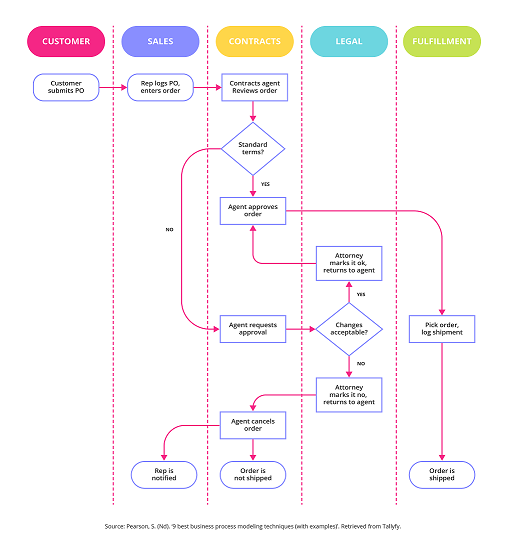
\includegraphics{pic5.png}
	\label{fig:label4}
\end{figure}

\section*{\lr{DFD (Data Flow Diagram)}}
\begin{itemize}
	\item \textbf{چه چیزهایی را مدل می‌کند:} جریان داده‌ها و ارتباطات بین فرایندها، داده‌ها و ذخیره‌سازی‌ها.
	\item \textbf{چگونگی مدل‌سازی:} با استفاده از نمودارهای گرافیکی برای نشان دادن جریان داده‌ها.
	\item \textbf{زمان استفاده:} در مراحل اولیه تحلیل سیستم برای درک بهتر جریان اطلاعات.
	\item \textbf{سطح انتزاع:} سطح بالا در ارتباط با جریان داده‌ها.
\end{itemize}

\section*{\lr{UML (Unified Modeling Language)}}
\begin{itemize}
	\item \textbf{چه چیزهایی را مدل می‌کند:} ساختار و رفتار سیستم‌های نرم‌افزاری.
	\item \textbf{چگونگی مدل‌سازی:} با استفاده از مجموعه‌ای متنوع از نمودارها (مانند نمودار کلاس، نمودار توالی).
	\item \textbf{زمان استفاده:} در تمام مراحل توسعه نرم‌افزار.
	\item \textbf{سطح انتزاع:} متغیر، بسته به نوع نمودار.
\end{itemize}

\section*{\lr{User Story}}
\begin{itemize}
	\item \textbf{چه چیزهایی را مدل می‌کند:} نیازمندی‌ها و ویژگی‌های کاربران از دیدگاه آن‌ها.
	\item \textbf{چگونگی مدل‌سازی:} به صورت جملات ساده و قابل فهم برای توصیف داستان‌های کاربری.
	\item \textbf{زمان استفاده:} بیشتر در رویکردهای توسعه چابک.
	\item \textbf{سطح انتزاع:} بسیار بالا و کاربر محور.
\end{itemize}

\section*{\lr{CRC Card (Class-Responsibility-Collaboration)}}
\begin{itemize}
	\item \textbf{چه چیزهایی را مدل می‌کند:} وظایف، مسئولیت‌ها و همکاری‌های کلاس‌ها.
	\item \textbf{چگونگی مدل‌سازی:} با استفاده از کارت‌هایی که کلاس‌ها و وظایف آن‌ها را نمایش می‌دهند.
	\item \textbf{زمان استفاده:} در مرحله طراحی سیستم و تعریف مسئولیت‌های کلاس‌ها.
	\item \textbf{سطح انتزاع:} متوسط تا بالا در ارتباط با ساختار کلاس‌ها.
\end{itemize}

\section*{\lr{BPMN (Business Process Model and Notation)}}
\begin{itemize}
	\item \textbf{چه چیزهایی را مدل می‌کند:} فرایندهای کسب‌وکار و وظایف مرتبط.
	\item \textbf{چگونگی مدل‌سازی:} با استفاده از نمودارهای فرایندی و نشانه‌گذاری‌های استاندارد.
	\item \textbf{زمان استفاده:} برای تحلیل و بهبود فرایندهای کسب‌وکار.
	\item \textbf{سطح انتزاع:} بالا در ارتباط با فرایندهای سازمانی.
\end{itemize}


